\chapter{Diseño del sistema}
\label{ch:diseno}
Tras haber realizado el análisis del sistema previamente, en este capítulo se desarrolla más en detalle las parte internas del sistema, como son las relacionadas con la arquitectura del sistema (\autoref{sec:arquitectura}), donde se define la manera en la que se relacionan y comunican las distintas partes que componen el sistema. 

También se define la manera en la que se almacenan los datos (\autoref{sec:modelo}) y como son las interfaces que componen el sistema (\autoref{sec:interfaz}) con las que interactúa el usuario. 

Además lo definido a continuación sienta la base para poder comenzar el desarrollo e implementación del sistema que se define en los siguientes capítulos, \autoref{ch:implementacion} y \autoref{ch:pruebas}.

\section{Arquitectura del Sistema}\label{sec:arquitectura}
El sistema que se desarrolla en este proyecto sigue un patrón de desarrollo bien definido, Modelo-Vista-Controlador \cite{bucanek_model-view-controller_2009}, que nos permite separar de una manera clara las diferentes partes del sistema que hay que desarrollar. Esta arquitectura se compone de las siguientes partes:
\begin{itemize}
	\item \textbf{Modelo:} Parte encargada de la representación lógica de la información en el sistema, los mecanismos para acceder y almacenarla. Esta será la parte relacionada con la base de datos.
	\item \textbf{Vista:} Es la representación visual del sistema que se mostrará al usuario cuando utilice la aplicación.
	\item \textbf{Controlador:} Representa toda la lógica del sistema, tanto el procesamiento de las medidas como el tratamiento de las peticiones al servidor.
\end{itemize}

Esta separación en tres partes permite que se puedan desarrollar e implementar las 3 partes en paralelo, de manera que quede todo más modularizado y dado el caso se puedan modificar o remplazar sin problema. Como podría ser que quisiéramos cambiar la página web (vista) por otra diferente sin que haga falta modificar el modelo y controlador. 

Además, es ampliamente usado y se ha demostrado su eficacia en multitud de proyectos de software.
\pagebreak

En la \autoref{fig:mvc} se puede ver cuál es la relación entre las diferentes partes que lo componen, que son:
\begin{itemize}
	\item El usuario en primer lugar solicita al servidor que le mande la página web. También cuando visualice la web realizara solicitudes de servicios y contenidos que va visualizando.
	\item El controlador recibe las solicitudes del usuario y se comunica con la vista, para que mandar la parte visual del sistema al usuario y que puede realizar más solicitudes. Cuando necesita acceder a información o almacenarla se comunica con el modelo, para que se encargue este.
	\item El modelo almacena los datos y cuando se le solicita los manda o almacena.
	\item La vista envía al usuario la parte visual del sistema que le vaya diciendo el controlador que es el que se encarga de la parte lógica de la web.
\end{itemize}

\begin{figure}[H]
	\ffigbox[\FBwidth]
	{\caption{Diagrama Modelo-Vista-Controlador}
		\label{fig:mvc}}
	{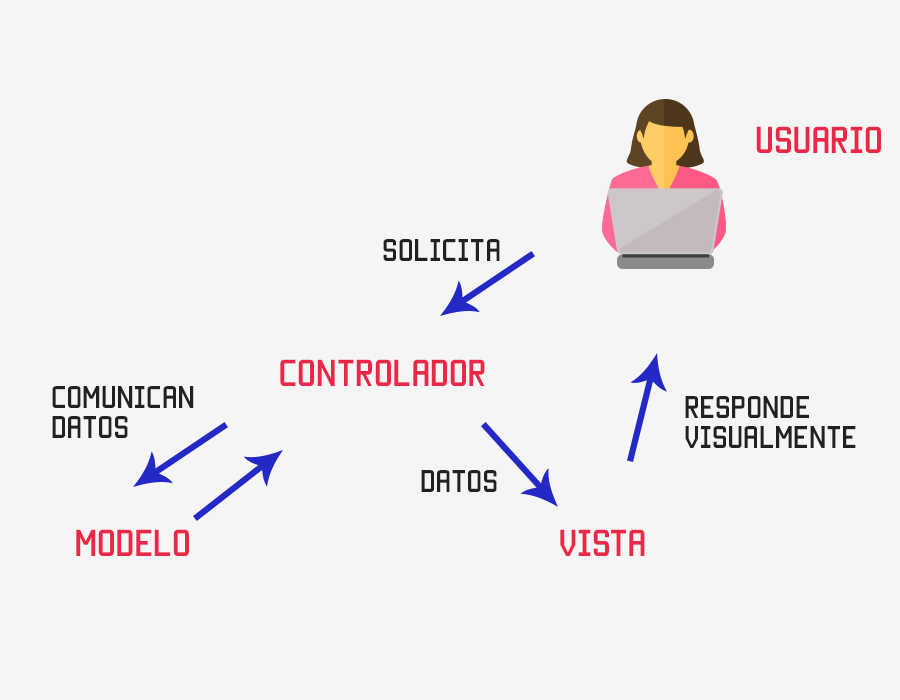
\includegraphics[scale=0.3]{mvc.jpg}}
\end{figure}

La manera en la que el usuario interactúa con el sistema será de Cliente-Servidor, lo que quiere decir que el usuario lo único que tendrá que hacer para utilizar el sistema será conectarse y acceder, será nuestro servidor el que tendrá todo el sistema y se encarga de responder todas las peticiones, gestionando los dispositivos, datos y web. 
\pagebreak

\section{Diagrama de Componentes}\label{sec:diagramaComponentes}
Esta sección se entra en más detalle cuál serán los componentes que conforman el sistema, en forma de diagrama de componentes, que se puede ver en la \autoref{fig:diagramaComponentes}.

Esta representación no permite definir de una manera estructurada y clara como se relacionan las diferentes partes del sistema, de manera que hay componentes que ofrecen interfaces a otros componentes y otros que las requieren para funcionar. Además, nos permite ver como fluye la información entre las diferentes partes del sistema y como estos la utilizan.
\begin{figure}[H]
	\ffigbox[\FBwidth]
	{\caption{Diagrama de Subsistemas y Componentes}
		\label{fig:diagramaComponentes}}
	{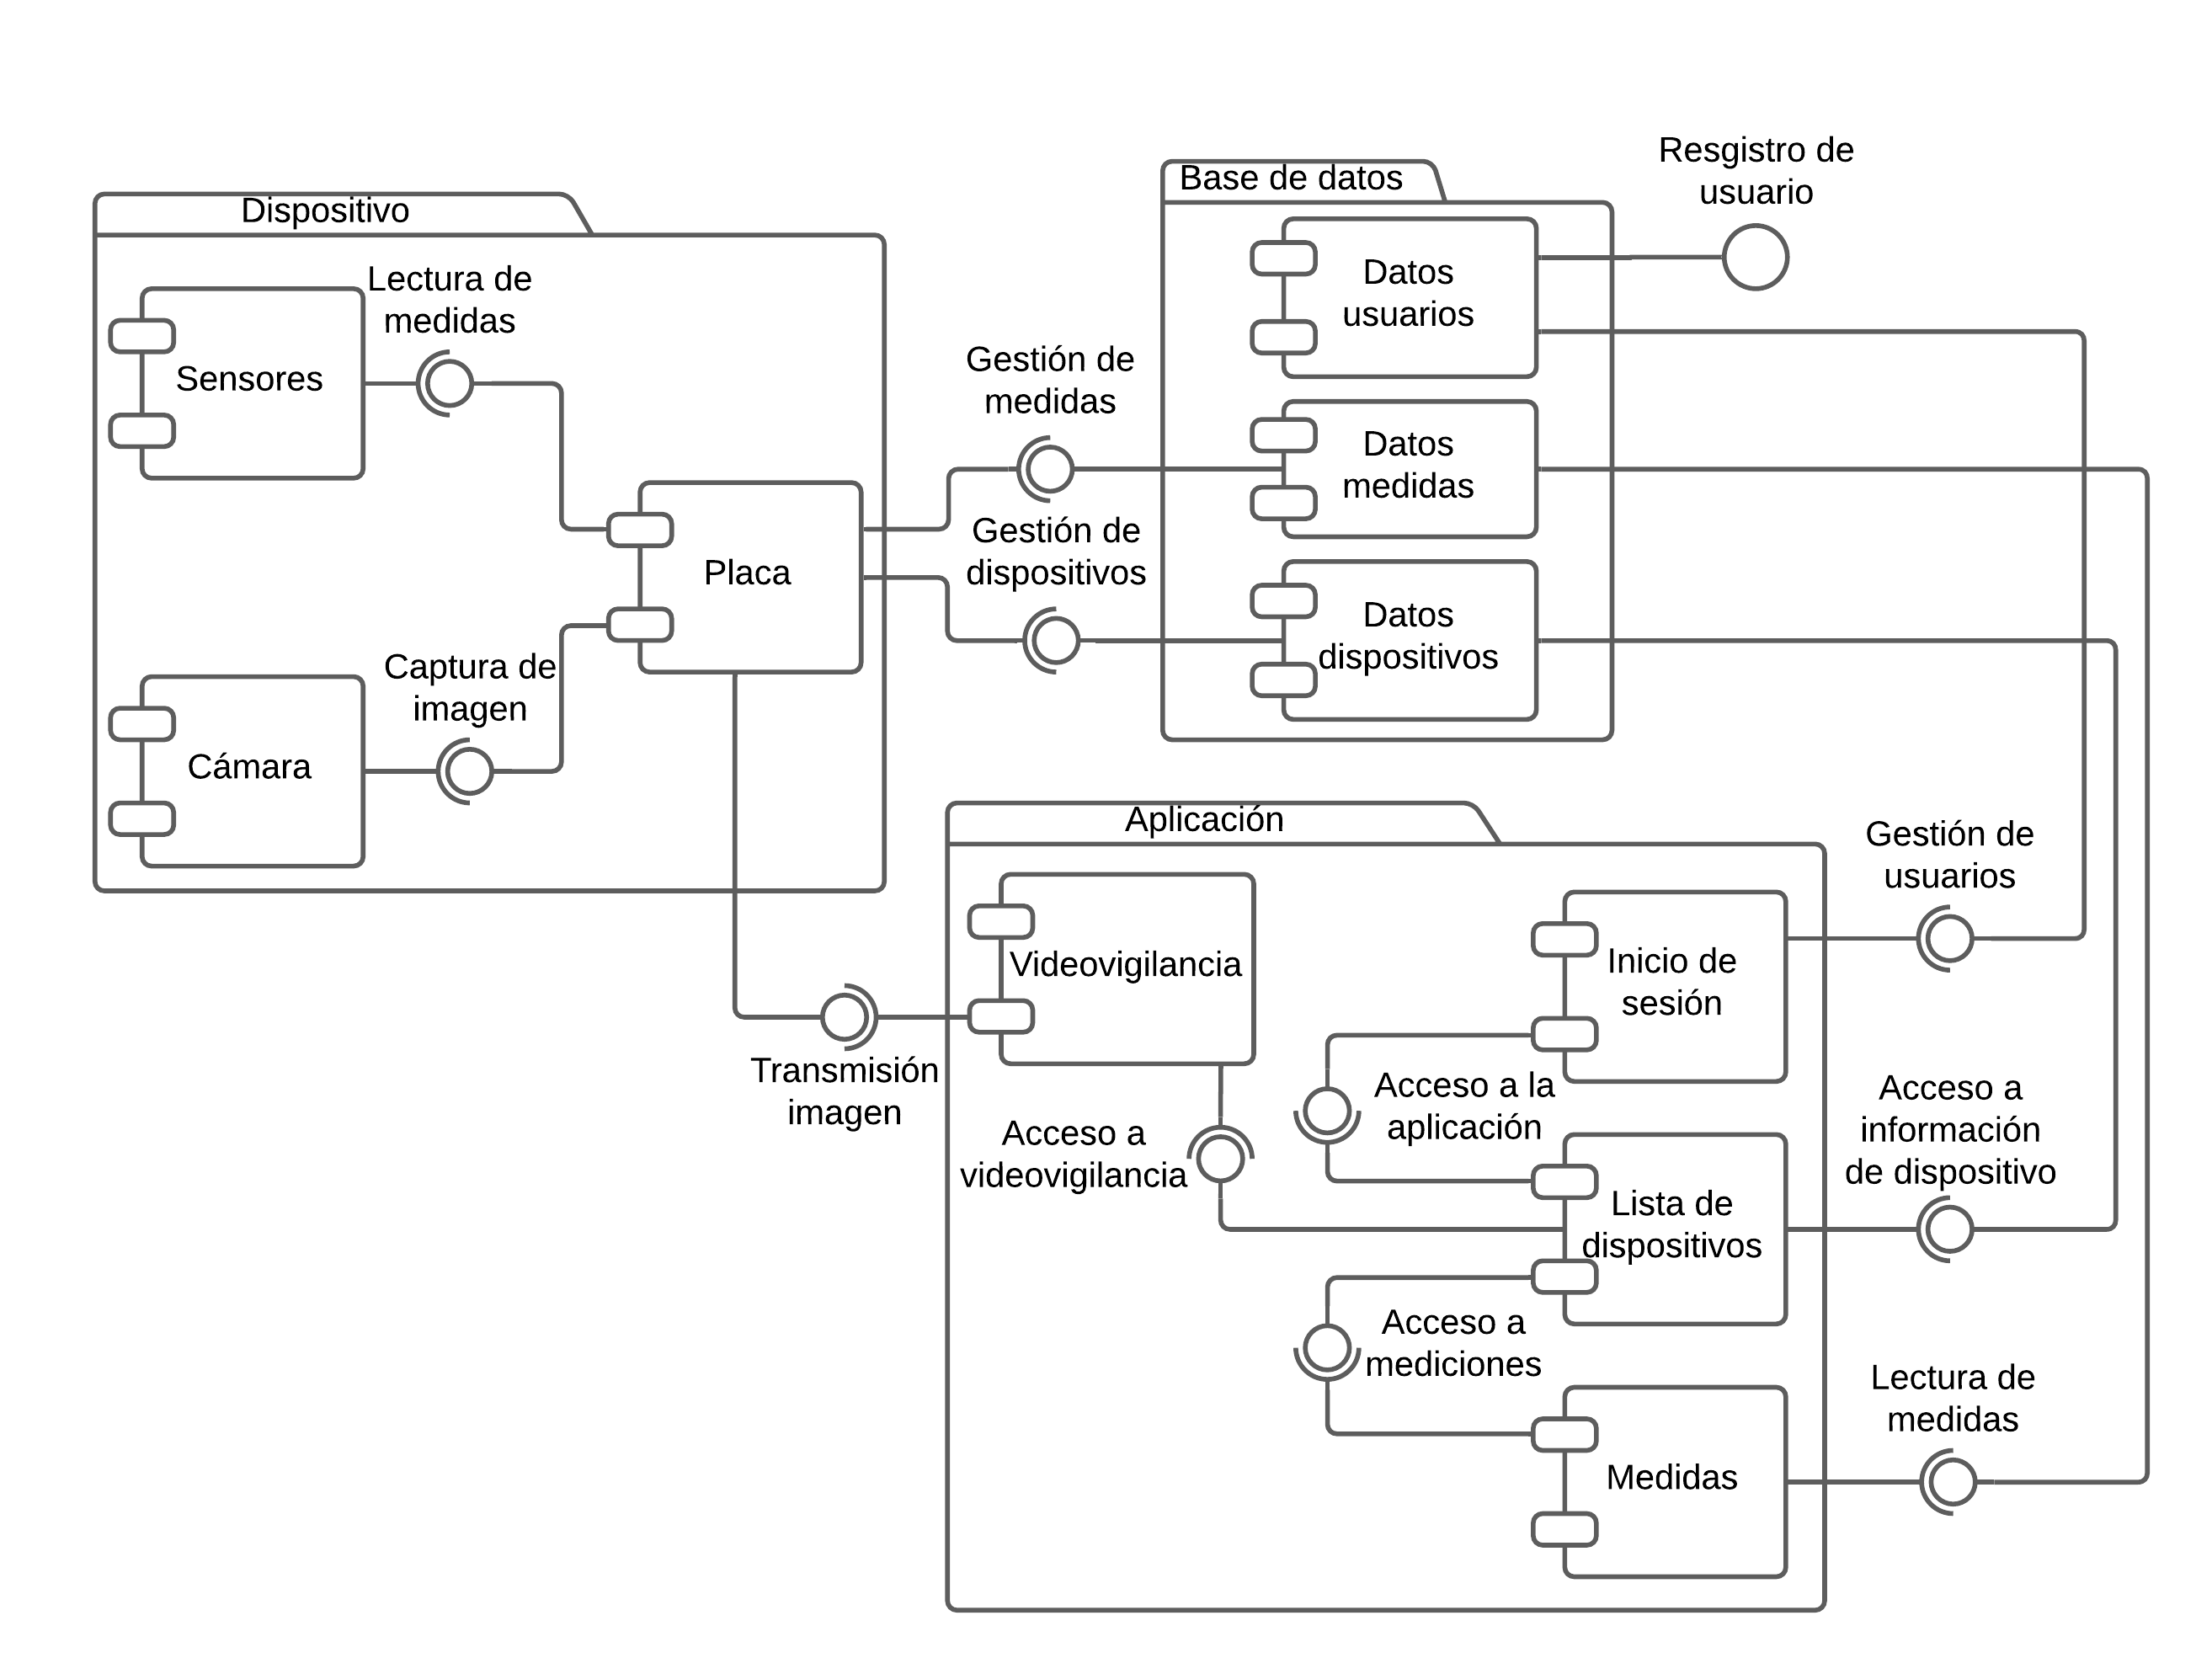
\includegraphics[scale=0.65]{diagramaComponentes.png}}
\end{figure}
Ahora se procede a explicar los subsistemas y componentes que lo forman:
\begin{itemize}
	\item \textbf{Dispositivo:} Representa a todos los dispositivos que se encuentra conectados al sistema y que tomaran las medidas del ambiente e imagen del interior de la sala, es por esto por lo que está formado por los siguientes componentes:
	      \begin{itemize}
		      \item \textbf{Sensores:} Cada uno de los componentes conectados al dispositivo que tomen medidas del ambiente. Estos están listos para ser empleados para leer las magnitudes correspondientes.
		      \item \textbf{Cámara:} Al igual que los sensores, esta será el componente conectado al dispositivo que se encargará de captar imagen del interior de la sala.
		      \item \textbf{Placa:} Componente clave del dispositivo que dentro del mismo recogerá las lecturas de los sensores y la imagen de la sala. Una vez tiene estos datos se encargará de enviar a la base de datos, a sus correspondientes componentes los datos de las medidas y los del propio dispositivo, además transmitirá la imagen de la cámara vía IP para que pueda ser recogida por la aplicación.
	      \end{itemize}
	\item \textbf{Base de datos:} Representa el conjunto de tablas que conforman la base de datos en la que se almacenarán las medidas, los datos del dispositivo y las credenciales de los usuarios. Sus componentes son:
	      \begin{itemize}
		      \item \textbf{Datos usuarios:} Es el componente encargado de almacenar las credencias de usuario, que se usaran para acceder a la aplicación, además permite que se introduzcan nuevos usuarios mediante su registro.
		      \item \textbf{Datos medidas:} Recibe las medidas de los dispositivos mediante la gestión de medidas y responde a las solicitudes de realizadas por la aplicación.
		      \item \textbf{Datos dispositivos:} Obtiene los datos de estado de los dispositivos que se encuentran en el sistema y da acceso a la aplicación a estos para ser mostrados.
	      \end{itemize}
	\item \textbf{Aplicación:} Es el subsistema con el que interactúa el usuario, al que mediante sus credenciales podrá acceder a ver los dispositivos conectados, sus medidas y la imagen que toman. Está compuesto por:
	      \begin{itemize}
		      \item \textbf{Inicio de sesión:} Es el componente que mediante la comprobación de las credenciales de usuario, permite acceder a la aplicación y estos son verificados mediante la base de datos.
		      \item \textbf{Lista de dispositivos:} Una vez se ha iniciado sesión en la aplicación, este nos permitirá ver los dispositivos conectados y su estado, que es obtenido de la base de datos.
		      \item \textbf{Medidas:} Es el encargado de mostrar de manera gráfica y tabular las diferentes medidas tomadas por el dispositivo de la lista de dispositivos, y estas medidas son obtenidas de la base de datos.
		      \item \textbf{Videovigilancia:} Es el componente encargado de mostrar la imagen en tiempo real del dispositivo instalado en la sala, recibe la imagen mediante la retransmisión del dispositivo y será accesible mediante la lista de dispositivos.
	      \end{itemize}
\end{itemize}

En las siguientes secciones se define la parte de Modelo (\autoref{sec:modelo}) y Controlador (\autoref{sec:interfaz}).
\pagebreak

\section{Modelo de datos}\label{sec:modelo}
En este proyecto la base de datos es uno de los elementos más importantes que lo componen, no solo para permitir el acceso del personal autorizado a la aplicación, sino porque almacenará el histórico de las medidas tomadas en la sala que en un futuro nos permitirá analizar cómo ha sido el estado de la sala.

La base de datos estará alojada en el servidor, donde podrá ser accedida por la aplicación más fácilmente para su visualización y consulta, además facilita que se puedan centralizar las medidas en un único lugar, para el caso de que se tuvieran múltiples dispositivos en un edificio y se deseara consultarlos desde un mismo lugar.

Como se comentó en la \autoref{subsec:servidorDB} se utiliza una base de datos MariaDB que se administra mediante phpMyAdmin \cite{noauthor_phpmyadmin_nodate}, que es un administrador de base de datos escrito en PHP, para realizar la mayoría de las tareas de una manera más sencilla y eficiente.

\subsection{Estructura de tablas de la base de datos}
Se presentan en esta subsección las tablas que componen la base de datos, indicando la utilidad de cada una de ellas y los datos con sus tipos que se almacenan en ellas. Antes de pasar a explicarlas en más detalle en la \autoref{fig:distDB} se puede ver un resumen de estas.
\begin{figure}[H]
	\ffigbox[\FBwidth]
	{\caption{Distribución de tablas en la base de datos}
		\label{fig:distDB}}
	{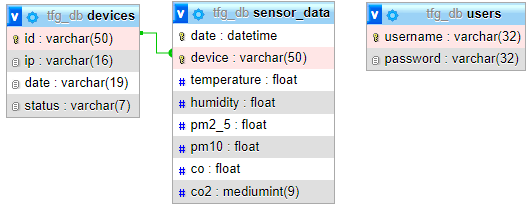
\includegraphics[scale=0.85]{db_dist.png}}
\end{figure}
\subsubsection{Tabla de usuarios}
En esta tabla se almacenarán las credenciales de los usuarios que utilicen la aplicación. Estas credenciales se consultarán cuando un usuario trata de iniciar sesión, y serán añadidos por el administrador del sistema en esta tabla. Es importante destacar que la contraseña se almacena en formato hash (encriptada) para evitar que se pueda leer si llega a haber cualquier intruso. 
\pagebreak

A continuación, en la \autoref{tab:tabla_users} se muestra la estructura de la tabla:
\begin{table}[H]
	\centering
	\caption{Estructura tabla users}
	\label{tab:tabla_users}
	\resizebox{\textwidth}{!}{%
		\begin{tabular}{|p{.2\textwidth}|p{.2\textwidth}|p{.6\textwidth}|}
			\hline
			\rowcolor[HTML]{BFBFBF}
			\multicolumn{1}{|c|}{\cellcolor[HTML]{BFBFBF}{\color[HTML]{000000} \textbf{Nombre}}} & \multicolumn{1}{c|}{\cellcolor[HTML]{BFBFBF}{\color[HTML]{000000} \textbf{Tipo}}} & \multicolumn{1}{c|}{\cellcolor[HTML]{BFBFBF}{\color[HTML]{000000} \textbf{Descripción}}} \\ \hline
			username                                                                             & varchar(32)                                                                       & Nombre de usuario que identifica unívocamente al usuario                                 \\ \hline
			password                                                                             & varchar(32)                                                                       & MD5 de la clave de acceso que debe proporcionar para verificar su identidad              \\ \hline
		\end{tabular}%
	}
\end{table}
La clave primaria será en username de esta manera no habrá ningún problema de duplicidad de usuarios en la base de datos.

\subsubsection{Tabla de dispositivos}
En esta tabla se almacenarán los dispositivos que se han conectado con el servidor, estos dispositivos serán los que se puedan consultar desde la aplicación y que se mostrarán con la fecha de actualización junto con su estado actual.

En la \autoref{tab:tabla_devices} se pueden ver los atributos que la componen:

\begin{table}[H]
	\centering
	\caption{Tabla devices BBDD}
	\label{tab:tabla_devices}
	\resizebox{\textwidth}{!}{%
		\begin{tabular}{|p{.2\textwidth}|p{.2\textwidth}|p{.6\textwidth}|}
			\hline
			\rowcolor[HTML]{BFBFBF}
			\multicolumn{1}{|c|}{\cellcolor[HTML]{BFBFBF}{\color[HTML]{000000} \textbf{Nombre}}} & \multicolumn{1}{c|}{\cellcolor[HTML]{BFBFBF}{\color[HTML]{000000} \textbf{Tipo}}} & \multicolumn{1}{c|}{\cellcolor[HTML]{BFBFBF}{\color[HTML]{000000} \textbf{Descripción}}} \\ \hline
			id                                                                                   & varchar(50)                                                                       & Nombre identificativo del dispositivo, su dirección física                               \\ \hline
			ip                                                                                   & varchar(16)                                                                       & IP de la red local desde la que se puede acceder a sus datos                             \\ \hline
			date                                                                                 & datetime                                                                          & Fecha de la última actualización de estado                                               \\ \hline
			status                                                                               & varchar(7)                                                                        & Estado del dispositivo, Online u Offline                                                 \\ \hline
		\end{tabular}%
	}
\end{table}
Como en la \autoref{tab:tabla_users} la clave primaria de la tabla es un nombre representativo, en este caso id, que identifica inequívocamente al dispositivo, de esta manera se puede utilizar para consultar los datos de un dispositivo en concreto. Cuando sea necesario puede variar la IP a la que está conectado, fecha y estado, pero el nombre identificador no puede cambiar.

\subsubsection{Tabla de medidas}
Es la tabla tan importante que se ha dicho antes, en esta tabla se almacenaran las medidas que han tomado todos los dispositivos conectados. Estos datos son los que se muestran en la página del dispositivo dentro de la aplicación junto con su imagen. Las medidas que se almacenan son: temperatura, humedad, PM2.5, PM10, CO y CO$_2$.

Los datos que la componen se exponen en la \autoref{tab:tabla_sensor_data}:

\begin{table}[H]
	\centering
	\caption{Tabla sensor\_data BBDD}
	\label{tab:tabla_sensor_data}
	\resizebox{\textwidth}{!}{%
		\begin{tabular}{|p{.2\textwidth}|p{.2\textwidth}|p{.6\textwidth}|}
			\hline
			\rowcolor[HTML]{BFBFBF}
			\multicolumn{1}{|c|}{\cellcolor[HTML]{BFBFBF}{\color[HTML]{000000} \textbf{Nombre}}} & \multicolumn{1}{c|}{\cellcolor[HTML]{BFBFBF}{\color[HTML]{000000} \textbf{Tipo}}} & \multicolumn{1}{c|}{\cellcolor[HTML]{BFBFBF}{\color[HTML]{000000} \textbf{Descripción}}} \\ \hline
			date                                                                                 & datetime                                                                          & Fecha en la que se ha tomado la medida                                                   \\ \hline
			device                                                                               & varchar(50)                                                                       & Identificador del dispositivo que captó la medida                                        \\ \hline
			temperature                                                                          & float                                                                             & Temperatura de la sala                                                                   \\ \hline
			humidity                                                                             & float                                                                             & Humedad de la sala                                                                       \\ \hline
			pm2\_5                                                                               & float                                                                             & Cantidad de partículas de 2.5$\mu m$ en la sala                                          \\ \hline
			pm10                                                                                 & float                                                                             & Cantidad de partículas de 10$\mu m$ en la sala                                           \\ \hline
			co                                                                                   & float                                                                             & Partículas por millón de CO en la sala                                                   \\ \hline
			co2                                                                                  & mediumint(9)                                                                      & Porcentaje de CO$_2$ en el aire de la sala                                               \\ \hline
		\end{tabular}%
	}
\end{table}
Las claves primarias son date y device, estas claves identifican de manera única a una medida, por lo que se puede consultar una medida concreta de un dispositivo específico.

Además, existe una relación con la tabla devices en cuanto a que el campo device es clave ajena del campo id, de esta manera que cuando un dispositivo sea eliminado o actualizado se propague a esta tabla.

\section{Interfaz de Usuario}\label{sec:interfaz}
En esta sección se trata otro de los elementos clave del sistema, la interfaz de usuario. Esta hace posible el uso del sistema a personas no expertas, de manera que puedan manipularlo y hacer uso de este sin la necesidad de saber cómo se desarrolla un sistema de estas características.

La parte del sistema a la que ha dotado de interfaz es la responsable de mostrar las medidas y video de las salas, tal y como ha solicitado el cliente. Para lograr esto se utiliza una página web, que se ha diseñado en HTML y CSS, con la que se puede acceder a toda esta información de una manera sencilla y visual. En cuanto a la lógica para obtener la información y movernos por las pantallas se emplea PHP.

La web además es responsive por lo que es totalmente funcional tanto en dispositivos de altas resoluciones (televisiones, ordenadores de sobremesa, portátiles, etc.), como en dispositivos de bajas resoluciones (móviles, tablets, etc.).

En la \autoref{fig:flujo_interfaz} se muestra el flujo de pantallas e interacciones que se sigue al acceder a la aplicación web, más tarde se explica en detalle cada una de las pantallas de la interfaz y que interacciones nos permite.
\begin{figure}[H]
	\ffigbox[\FBwidth]
	{\caption{Diagrama de flujo de la web}
		\label{fig:flujo_interfaz}}
	{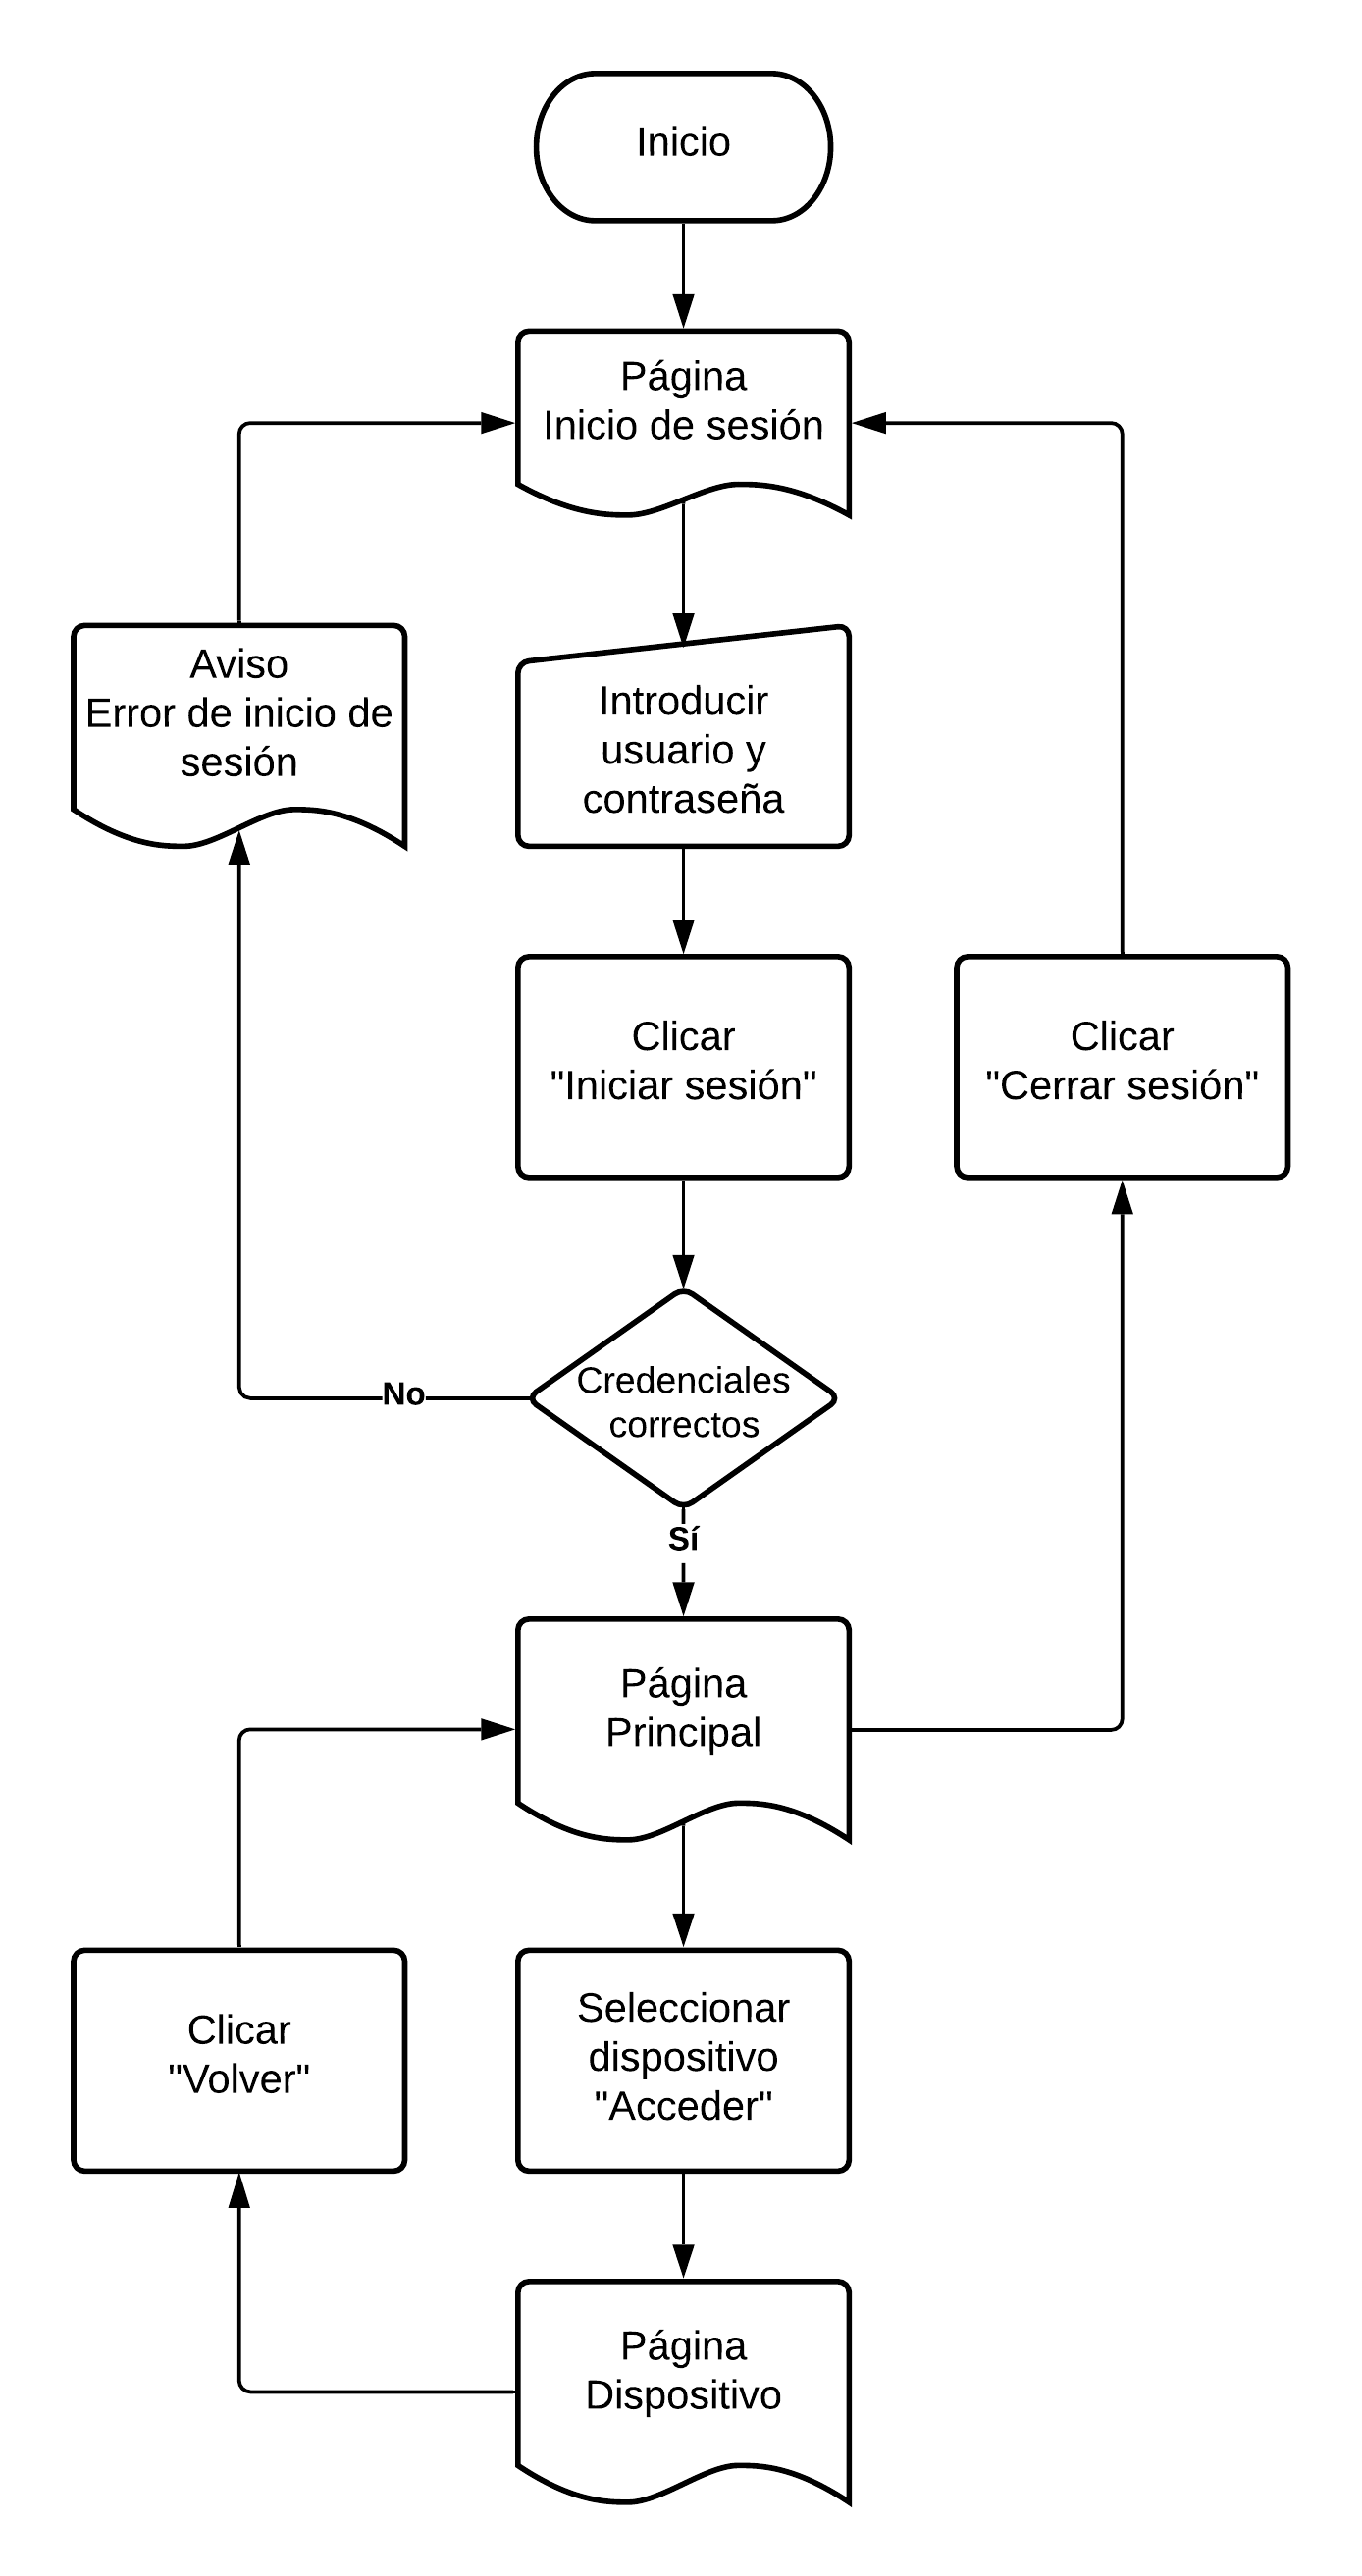
\includegraphics[scale=0.9]{flujoInterfaz.png}}
\end{figure}

\subsection{Página: Inicio de sesión}
Es la primera pantalla que se encontrara el usuario cuando acceda a la aplicaccion, en esta, como se puede ver en la ILUSTRACION XX se le solicita intrudicir su nombre  de usuario y contraseña de acceso. Esta pantalla es fundamental para garantizar la seguridad del centro, de manera que no accedan personas no autorizadas y que puedan poner en riesgo su seguridad.

Se puede ver de primeras que la paleta de colores se adapta a lo solicitado, utilizando colores de la gama de los azules que contratesn entre ellos, de manera que se pueda visualizar sin difultad todos los elementos, los codigos elegidos han sido:
PONER LOS COLORES USADOS

El primer campo, correspondiente al nombre de usuario se muestra el texto escrito, sin embargo en el de la contraseña se sustituiran visualmente por asteriscos garantizando la provacidad de la contraseña.

En el caso de introducor unos credenciales no resgistrados en el sistema se avisa al usuario de que recise lo que ha escrito, dado que si no coinciden no se puede garantizar si identidad.

Por otro lado, tambien se deben completar ambos campos, si esto no es así se lanza un aviso al usuario informandole que los debe cumplimentar si desea acceder.

Una vez el usuario ha completado los campos podrá hacer clic en el boton "Iniciar sesión" que si cumple todo los anterior le llevara a la pantalla principal descita en la SUBSECCION XX

En cuanto a la versión movil, se ha ajustado el tamaño del formaulario para que se ajuste y sea legible incluso en resoluciones pequeñas. Además el tamaño de letra es suficientemente grande como para que se pueda leer correctamente tanto en grandes como en pequenas resoluciones. PONER TAMANO LETRA

\subsection{Página: Principal}
Una vez el usuario a iniciado la sesion de manera satisfactoria, se pasara a la panatalla mostrada en la ILUSTRACION XX, en la que de primera podemos ver que nos muestra un mesaje de saludo, indicando el nombre de usuario.

La clave de esta pantalla es la lista de los dispositivos en la que se muestran de manera tabular los datos de estos. Se imprimiran para cada dispositivo los datos almacenados en la base de datos.

En la ultima posicion de cada fila de dipositivo hay un boton en el que pone "Acceso" que nos redirigira a la pagina de dispositivo, que se describe en la SUBSECCION XX.

En la parte inferior aparece un boton con el texto "Cerrar sesion" que como su propio nombre indica, cierra la sesion y nos devuelve a la pagina de inicio de sesion, SUBSECCION XX.

Por ultimo, en la version movil la tabla pasara a ocupar el ancho completo de la pantalla para que se pueda ver claraemnte el boton de la ultima posicion y facilitar acceder al dispositivo. En cuanto al texto de saludo se ha decidido mantener, pero ajustandose para que no se salga de la pantalla, evitando el scroll lateral.

\subsection{Página: Dispositivo}
Esta pantalla muestra la informacion clave de este proyecto, la imagen de la camara del dispositovo y las medidas tomadas. 

A esta pagina se acceder una vez se ha seleccionado un dispositivo en la pagina principal, SUBSECCION XX, y tiene la apariencia que se muestra en la ILUSTRACION XX.

En primer lugar, en la parte superior se muestra el nombre que identifica al dispositivo de manera que podemos saber en todo momento que datos estamos consultado.

Inmediatamente despues, se muestra un cuadro con la imagen en tiempo real de la camara del dispositivo.

A continuacion, se mostraran todas la medidas, primero de manera grafica y despues de manera tabular. 

La parte de medidas en forma de graficas se divide en 3 apartados XXXX

En cuanto a la forma tabular, mediante una tabla se muestran las medidas de manera cronologica, de mas nuevas a mas antiguas. Esta tabla esta compuesta por los XXX ultimos resgistros que cubren la ultima hora de mediciones de la sala.


Poner capturas y hablar en general, después poner las imágenes de móvil y explicar que se ha hecho para que sea responsive(dimensiones adaptables, tamaños de letra, contraste).
